%% LyX 2.1.2.1 created this file.  For more info, see http://www.lyx.org/.
%% Do not edit unless you really know what you are doing.
\documentclass[english]{beamer}
\usepackage[T1]{fontenc}
\usepackage[latin9]{inputenc}
\setcounter{secnumdepth}{3}
\setcounter{tocdepth}{3}
\usepackage{mathrsfs}
\usepackage{amssymb}
\usepackage{subcaption}
\captionsetup{compatibility=false}

\makeatletter
%%%%%%%%%%%%%%%%%%%%%%%%%%%%%% Textclass specific LaTeX commands.
 % this default might be overridden by plain title style
 \newcommand\makebeamertitle{\frame{\maketitle}}%
 % (ERT) argument for the TOC
 \AtBeginDocument{%
   \let\origtableofcontents=\tableofcontents
   \def\tableofcontents{\@ifnextchar[{\origtableofcontents}{\gobbletableofcontents}}
   \def\gobbletableofcontents#1{\origtableofcontents}
 }

%%%%%%%%%%%%%%%%%%%%%%%%%%%%%% User specified LaTeX commands.
\beamertemplateshadingbackground{red!5}{structure!5}

\usepackage{beamerthemeshadow}
\usepackage{pgfnodes,pgfarrows,pgfheaps}

\beamertemplatetransparentcovereddynamicmedium






\newcommand{\Class}[1]{\operatorname{\mathchoice
  {\text{\small #1}}
  {\text{\small #1}}
  {\text{#1}}
  {\text{#1}}}}

\newcommand{\Lang}[1]{\operatorname{\text{\textsc{#1}}}}

\newcommand{\tape}[3]{%
  \color{structure!30!bg}
  \pgfmoveto{\pgfxy(-0.5,0)}
  \pgflineto{\pgfxy(-0.6,0.1)}
  \pgflineto{\pgfxy(-0.4,0.2)}
  \pgflineto{\pgfxy(-0.6,0.3)}
  \pgflineto{\pgfxy(-0.4,0.4)}
  \pgflineto{\pgfxy(-0.5,0.5)}
  \pgflineto{\pgfxy(4,0.5)}
  \pgflineto{\pgfxy(4.1,0.4)}
  \pgflineto{\pgfxy(3.9,0.3)}
  \pgflineto{\pgfxy(4.1,0.2)}
  \pgflineto{\pgfxy(3.9,0.1)}
  \pgflineto{\pgfxy(4,0)}
  \pgfclosepath
  \pgffill

  \color{structure}  
  \pgfputat{\pgfxy(0,0.7)}{\pgfbox[left,base]{#1}}
  \pgfputat{\pgfxy(0,-0.1)}{\pgfbox[left,top]{#2}}

  \color{black}
  \pgfputat{\pgfxy(-.1,0.25)}{\pgfbox[left,center]{\texttt{#3}}}%
}

\newcommand{\shorttape}[3]{%
  \color{structure!30!bg}
  \pgfmoveto{\pgfxy(-0.5,0)}
  \pgflineto{\pgfxy(-0.6,0.1)}
  \pgflineto{\pgfxy(-0.4,0.2)}
  \pgflineto{\pgfxy(-0.6,0.3)}
  \pgflineto{\pgfxy(-0.4,0.4)}
  \pgflineto{\pgfxy(-0.5,0.5)}
  \pgflineto{\pgfxy(1,0.5)}
  \pgflineto{\pgfxy(1.1,0.4)}
  \pgflineto{\pgfxy(0.9,0.3)}
  \pgflineto{\pgfxy(1.1,0.2)}
  \pgflineto{\pgfxy(0.9,0.1)}
  \pgflineto{\pgfxy(1,0)}
  \pgfclosepath
  \pgffill

  \color{structure}  
  \pgfputat{\pgfxy(0.25,0.7)}{\pgfbox[center,base]{#1}}
  \pgfputat{\pgfxy(0.25,-0.1)}{\pgfbox[center,top]{#2}}

  \color{black}
  \pgfputat{\pgfxy(-.1,0.25)}{\pgfbox[left,center]{\texttt{#3}}}%
}

\pgfdeclareverticalshading{heap1}{\the\paperwidth}%
  {color(0pt)=(black); color(1cm)=(structure!65!white)}
\pgfdeclareverticalshading{heap2}{\the\paperwidth}%
  {color(0pt)=(black); color(1cm)=(structure!55!white)}
\pgfdeclareverticalshading{heap3}{\the\paperwidth}%
  {color(0pt)=(black); color(1cm)=(structure!45!white)}
\pgfdeclareverticalshading{heap4}{\the\paperwidth}%
  {color(0pt)=(black); color(1cm)=(structure!35!white)}
\pgfdeclareverticalshading{heap5}{\the\paperwidth}%
  {color(0pt)=(black); color(1cm)=(structure!25!white)}
\pgfdeclareverticalshading{heap6}{\the\paperwidth}%
  {color(0pt)=(black); color(1cm)=(red!35!white)}

\newcommand{\heap}[5]{%
  \begin{pgfscope}
    \color{#4}
    \pgfheappath{\pgfxy(0,#1)}{\pgfxy(-#2,0)}{\pgfxy(#2,0)}
    \pgfclip
    \begin{pgfmagnify}{1}{#1}
      \pgfputat{\pgfpoint{-.5\paperwidth}{0pt}}{\pgfbox[left,base]{\pgfuseshading{heap#5}}}
    \end{pgfmagnify}
  \end{pgfscope}
  %\pgffill
  
  \color{#4}
  \pgfheappath{\pgfxy(0,#1)}{\pgfxy(-#2,0)}{\pgfxy(#2,0)}
  \pgfstroke

  \color{white}
  \pgfheaplabel{\pgfxy(0,#1)}{#3}%
}


\newcommand{\langat}[2]{%
  \color{black!30!beamerexample}
  \pgfsetlinewidth{0.6pt}
  \pgfsetendarrow{\pgfarrowdot}
  \pgfline{\pgfxy(-3.5,#1)}{\pgfxy(0.05,#1)}
  \color{beamerexample}
  \pgfputat{\pgfxy(-3.6,#1)}{\pgfbox[right,center]{#2}}%
}

\newcommand{\langatother}[2]{%
  \color{black!30!beamerexample}
  \pgfsetlinewidth{0.6pt}
  \pgfsetendarrow{\pgfarrowdot}
  \pgfline{\pgfxy(3.5,#1)}{\pgfxy(-0.05,#1)}
  \color{beamerexample}
  \pgfputat{\pgfxy(3.6,#1)}{\pgfbox[left,center]{#2}}%
}


\pgfdeclaremask{knight1-mask}{beamer-knight1-mask} \pgfdeclareimage[height=2cm,mask=knight1-mask]{knight1}{beamer-knight1} \pgfdeclaremask{knight2-mask}{beamer-knight2-mask} \pgfdeclareimage[height=2cm,mask=knight2-mask]{knight2}{beamer-knight2} \pgfdeclaremask{knight3-mask}{beamer-knight3-mask} \pgfdeclareimage[height=2cm,mask=knight3-mask,interpolate=true]{knight3}{beamer-knight3} \pgfdeclaremask{knight4-mask}{beamer-knight4-mask} \pgfdeclareimage[height=2cm,mask=knight4-mask,interpolate=true]{knight4}{beamer-knight4}


\pgfdeclareradialshading{graphnode}
  {\pgfpoint{-3pt}{3.6pt}}%
  {color(0cm)=(beamerexample!15);
    color(2.63pt)=(beamerexample!75);
    color(5.26pt)=(beamerexample!70!black);
    color(7.6pt)=(beamerexample!50!black);
    color(8pt)=(beamerexample!10!bg)}

\newcommand{\graphnode}[2]{
  \pgfnodecircle{#1}[virtual]{#2}{8pt}
  \pgfputat{#2}{\pgfbox[center,center]{\pgfuseshading{graphnode}}}
}

\makeatother

\usepackage{babel}
\begin{document}

\title{Asymptotic Validity of the Bayes-Inspired Indifference Zone Procedure:
the Non-Normal Known Variance Case}


\author{Saul Toscano-Palmerin\\
Peter Frazier}


\institute{School of Operations Research and Information Engineering, Cornell
University\\
}


\date{June 14, 2015\\
}
\makebeamertitle
\begin{frame}{Indifference-Zone Ranking and Selection}

\begin{block}{}

\begin{itemize}
\item Ranking and Selection is a problem where we have to select the best
alternative among $\left\{ \mu_{1},\mu_{2},\ldots,\mu_{k}\right\} $
based on iid samples. \\
\textrm{}\\
\item If a procedure chooses $\hat{x}$, the probability of correct selection
is \[
\mbox{PCS}\left(\mu\right)=\mathbb{P}_{\mu}\left(\hat{x}\in\mbox{arg max}_{x}\mu_{x}\right).
\]\textrm{}\\
\item The preference zone is $\mbox{PZ}\left(\delta\right)=\left\{ \mu\in\mathbb{R}^{k}:\mu_{\left[k\right]}-\mu_{\left[k-1\right]}\geq\delta\right\} $.
\\
\textrm{}\\
\item A procedure meets the IZ guarantee at $P^{*}\in\left(1/k,1\right)$
and $\delta>0$ if 
\[
\mbox{PCS}\left(\mu\right)\geq P^{*}\mbox{ for all }\mu\in\mbox{PZ}\left(\delta\right).
\]
\\
\textrm{}\\
\end{itemize}
\end{block}
\end{frame}

\begin{frame}{Conservatism Causes the Number of Samples Taken to Be Larger than
Necessary }

\begin{block}{}

\begin{itemize}
\item A user wants to meet the IZ guarantee and have $\mathbb{E}\left[\mbox{\# of samples}\right]$
as small as possible.\\
\textrm{}\\
\item The conservatism can be defined as $\mbox{PCS}\left(\mu\right)-P^{*}$.
If this number is large, then $\mathbb{E}\left[\mbox{sample size}\right]$
may be large. 
\end{itemize}
\end{block}
\end{frame}



\begin{frame}{Sources of Conservatism}

\begin{block}{}

\begin{itemize}
\item The change from discrete time to continuous time often used to show
IZ guarantees.\\
\textrm{}\\
\item The configuration under consideration is not a worst-case configuration.
\\
\textrm{}\\
\item Bonferroni\textquoteright s inequality.
\end{itemize}
\end{block}
\end{frame}

\begin{frame}{The Bayes-Inspired IZ (BIZ) Procedure}

\begin{block}{}

\begin{itemize}
\item BIZ is an elimination procedure that eliminates the use of Bonferroni\textquoteright s
inequality, reducing conservatism. \\
\textrm{}\\
\item Its lower bound on worst-case probability of correct selection in
the preference zone is tight in continuous time, and almost tight
in the discrete time.\\
\textrm{}\\
\item The number of samples required by BIZ is significantly smaller than
the KN procedure and the $\mathscr{P}_{B}^{*}$ procedure.\\
\textrm{}\\

\end{itemize}
\end{block}
\end{frame}

\begin{frame}{BIZ Requires Fewer Samples}
\begin{figure}[ht]
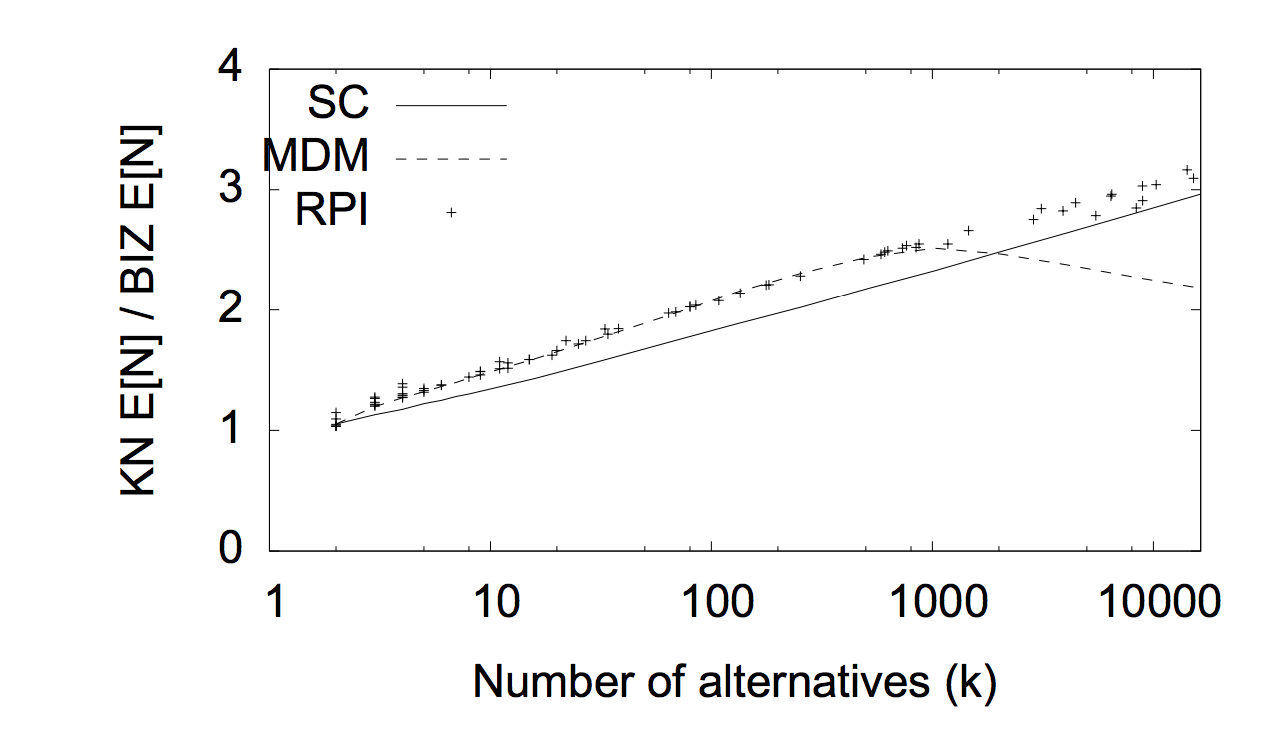
\includegraphics[width=\textwidth,height=0.8\textheight,keepaspectratio]{BIZ.png}
\end{figure}
\end{frame}

\begin{frame}{The Bayes-Inspired IZ (BIZ) Procedure}

\begin{block}{}

\begin{itemize}
\item It satisfies the IZ guarantee under the following assumptions:

\begin{itemize}
\item Normal samples.\\

\item Known variances.\\

\item Variances are either common across alternatives, or have an integer
multiple structure.\\
\textrm{}\\
\end{itemize}
\item Based on empirical evidence, the BIZ procedure satisfies the IZ guarantee
almost always even when the last two assumptions are not true.\\
\textrm{}\\
\item Our contribution is to theoretically explain why it works. Specifically,
we show asymptotic validity of the BIZ procedure. 
\end{itemize}
\end{block}
\end{frame}

\begin{frame}{Asymptotic Validity}

\begin{block}{Theorem}
 If samples are iid and the variances are finite and do not depend
on $\delta$, then 

\[
\mbox{inf }_{a\in\mbox{PZ}\left(1\right)}\mbox{lim}_{\delta\rightarrow0^{+}}\mbox{PCS}\left(\delta\right)=P^{*}
\]
where $\mu_{k}=a_{k}\delta,\ldots,\mu_{1}=a_{1}\delta.$ 
\end{block}
\end{frame}

\begin{frame}{The Bayes-Inspired IZ (BIZ) Procedure}

\begin{block}{}


The BIZ procedure can be viewed as the composition of three maps:\\
\textrm{}\\

\end{block}
\begin{itemize}
\item The mapping from $\left(Y_{tx}:t\in\mathbb{N},x\in\left\{ 1,\ldots,k\right\} \right)$,
where $Y_{tx}$ is the sum of the first $t$ samples from alternative
$x$, onto $\left(Z_{tx}:t\in\mathbb{N},x\in\left\{ 1,\ldots,k\right\} \right)$
where $Z_{tx}=Y_{n_{tx},t}$ is the sum of samples from alternative
$x$observed by stage $t$.\\
\textrm{}\\
\item The second maps the previous time-changed random walk through a non-linear
mapping for each $t,x$ and subset $A\subset\left\{ 1,\ldots,k\right\} $,
to $\left(q_{tx}^{'}\left(A\right):t\in\mathbb{N},A\subset\left\{ 1,\ldots,k\right\} ,x\in A\right)$,
where
\[
q_{tx}^{'}\left(A\right)=\mbox{exp}\left(\delta\beta_{t}\frac{Z_{tx}}{n_{tx}}\right)\left/\sum_{x'\in A}\mbox{exp}\left(\delta\beta_{t}\frac{Z_{tx'}}{n_{tx'}}\right)\right.
\]

\end{itemize}
\end{frame}

\begin{frame}{The Bayes-Inspired IZ (BIZ) Procedure}

\begin{itemize}
\item The third map, $h$, maps the paths of $\left(q_{tx}^{'}\left(A\right):t\in\mathbb{N},A\subset\left\{ 1,\ldots,k\right\} ,x\in A\right)$
onto selection decisions.

\begin{itemize}
\item Finds first time $\tau_{1}$ that $q_{tx}^{'}\left(A_{0}\right)\geq P_{0}$
or $q_{tx}^{'}\left(A_{0}\right)\leq c$. In the first case, $x_{0}\in\mbox{arg max}_{x}q_{tx}^{'}\left(A_{0}\right)$
is selected as the best. In the second case, $x_{0}\in\mbox{arg min}_{x}q_{tx}^{'}\left(A_{0}\right)$
is eliminated from $A_{0}$, resulting in new parameters $A_{1}$
and $P_{1}$.\\
\textrm{}\\
\item This process is repeated until an alternative is selected as the best.\\
\textrm{}\\
\end{itemize}
\end{itemize}
\end{frame}

\begin{frame}{Proof Outline}

\begin{block}{}

\begin{itemize}
\item The same selection decision is obtained if we apply the map $h$ to
$\left(q_{tx}\left(A\right):t\in\delta^{2}\mathbb{N},A\subset\left\{ 1,\ldots,k\right\} ,x\in A\right)$
\inputencoding{latin1}{where $q_{tx}\left(A\right):=q^{'}\left(\left(Z_{\frac{t}{\delta^{2}}x}:x\in A\right),\delta,t\right)$.}\\
\inputencoding{latin9}\textrm{}\\
\item The discrete-time process is interpolated by the continuous-time process
$\left(q_{tx}\left(A\right):t\geq0,A\subset\left\{ 1,\ldots,k\right\} ,x\in A\right)$.\\
\textrm{}\\
\item The selection decision between the continuous-time process and the
discrete-time process goes to zero as $\delta\rightarrow0$.\\
\textrm{}\\
\item Applying the BIZ selection map $h$ to the previous process, produces
a selection decision that satisfies the indifference-zone guarantee
as $\delta\rightarrow0$.
\end{itemize}
\end{block}
\end{frame}





\begin{frame}{Proof Outline}

\begin{block}{}

\begin{itemize}
\item \inputencoding{latin1}The following centralized version of $Z_{\frac{t}{\delta^{2}}x}$
\[
\mathscr{C}_{x}\left(\delta,t\right):=\frac{Y_{n_{x}\left(t\right),x}-t\lambda_{x}^{2}\mu_{x}}{\frac{\lambda_{x}^{2}}{\lambda_{z}}\delta}
\]
converges to a Brownian motion as $\delta\rightarrow0$.\\
\inputencoding{latin9}\foreignlanguage{english}{\textrm{}\\}
\selectlanguage{english}%
\item We construct $f\left(\cdot,\delta\right)$ that takes as input the
process $\left(\mathscr{C}_{x}\left(\delta,t\right):x\in\left\{ 1,\ldots,k\right\} ,t\in\mathbb{R}\right)$,
and returns $1$ if the correction selection was made, and $0$ otherwise.\\
\textrm{}\\
\end{itemize}
\end{block}
\end{frame}

\begin{frame}{Proof Outline}

\begin{block}{}

\begin{itemize}
\item $f$ has a continuity property that causes $f\left(\mathscr{C}\left(\delta,\cdot\right),\delta\right)\Rightarrow g\left(W\right)$
where $g$ is the selection decision from applying the BIZ procedure
in continuous time.\inputencoding{latin1}{}\\
\inputencoding{latin9}\textrm{}\\
\item \inputencoding{latin1}The BIZ procedure satisfies the IZ guarantee
when applied in continuous time, and so $\mathbb{E}\left[g\left(W\right)\right]\geq P^{*}$
with equality for the worst configuration in the preference zone.\\
\inputencoding{latin9}\foreignlanguage{english}{\textrm{}\\}
\end{itemize}
\end{block}
\end{frame}

\begin{frame}{Numerical Experiments}
\begin{figure}[ht]
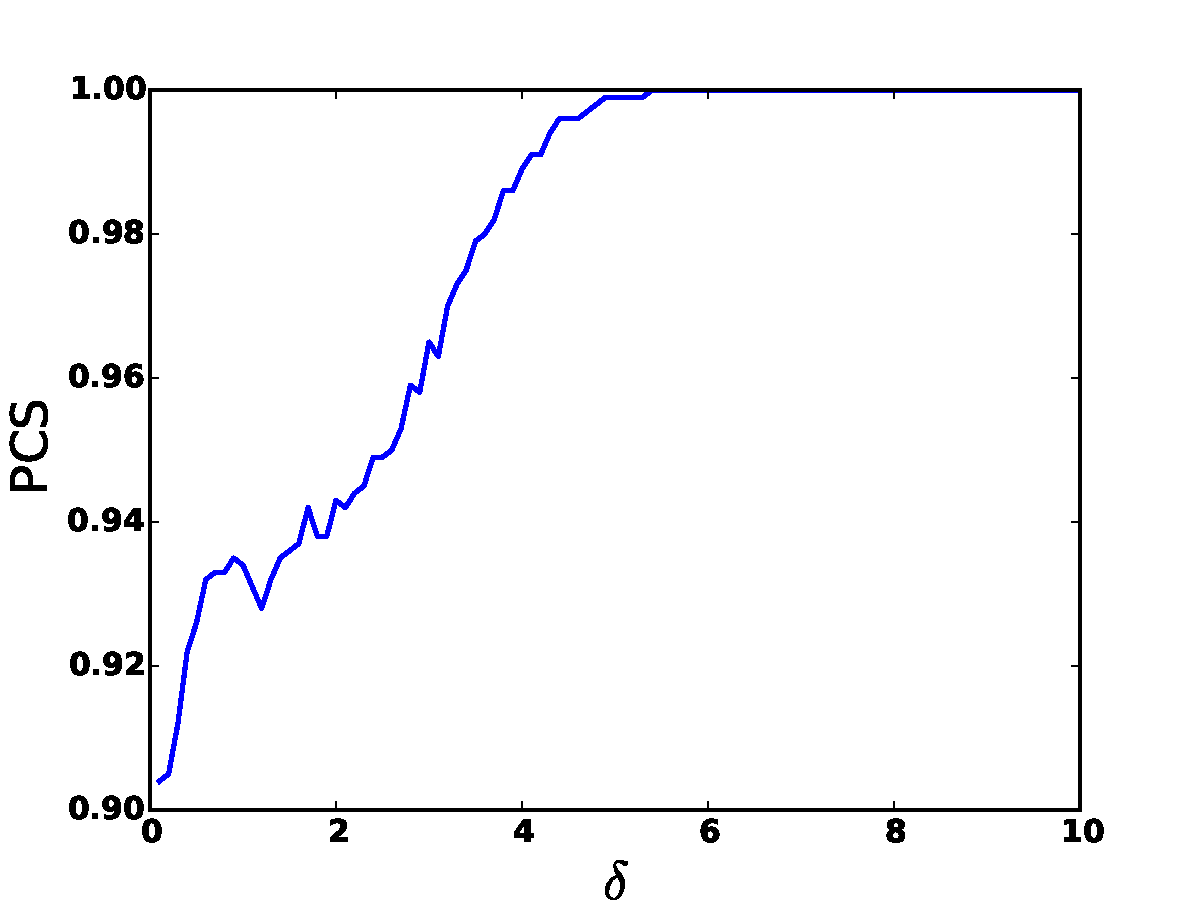
\includegraphics[width=\textwidth,height=0.7\textheight,keepaspectratio]{plot5.pdf}
\caption{
    Known variance case. 100 alternatives and $P^*=0.9$. PCS converges to $P^*$ as $\delta$ goes to $0$.
    Typical behavior, where the PCS is above $P^*$ for all values of $\delta$.}
\end{figure}
\end{frame}

\begin{frame}{Numerical Experiments}
\begin{figure}[ht]
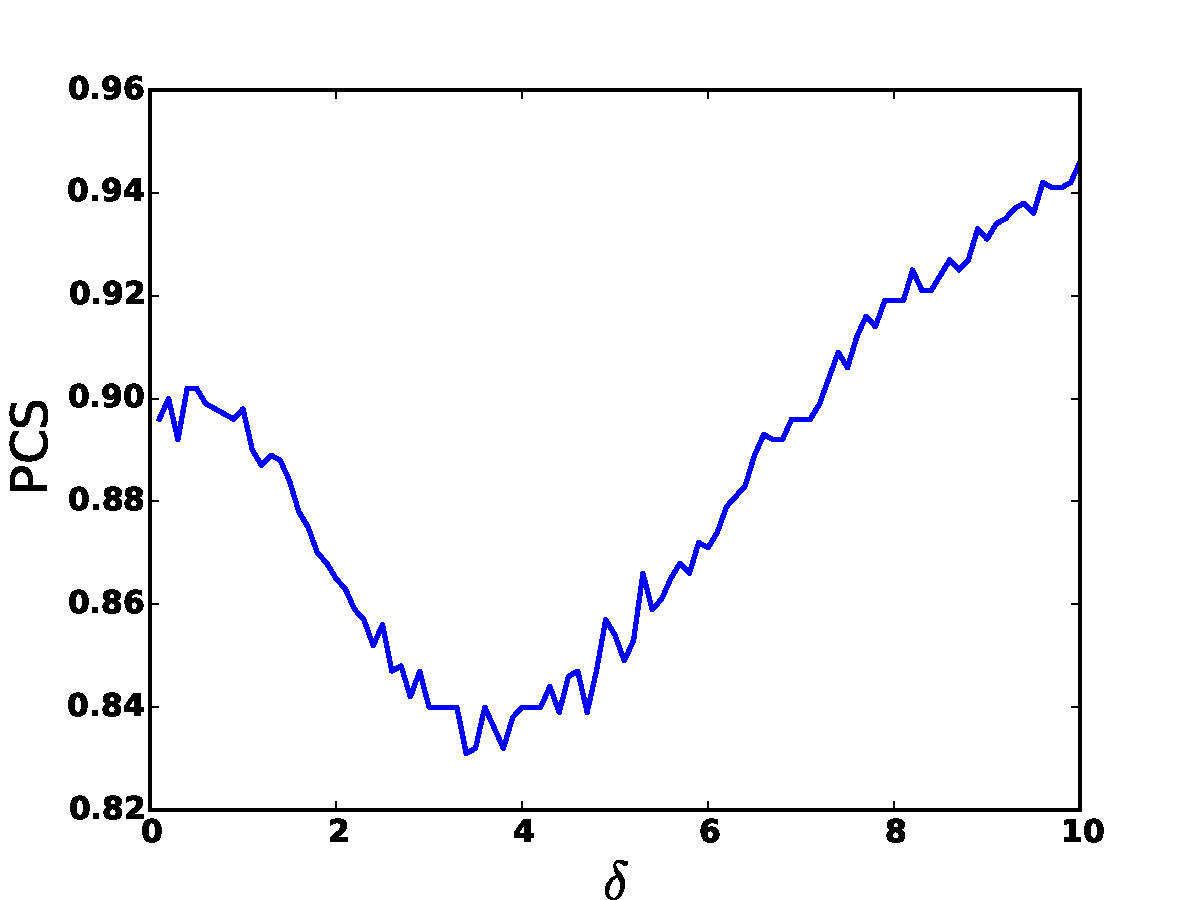
\includegraphics[width=\textwidth,height=0.7\textheight,keepaspectratio]{unknown.pdf}
\caption{
    Unknown variance case. 100 alternatives and $P^*=0.9$. PCS converges to $P^*$ as $\delta$ goes to $0$. 
    Atypical behavior, $n_0$ is small and the variance of the best alternative is much larger than the other variances.}
\end{figure}
\end{frame}

\begin{frame}{Numerical Experiments}
\begin{figure}[ht]
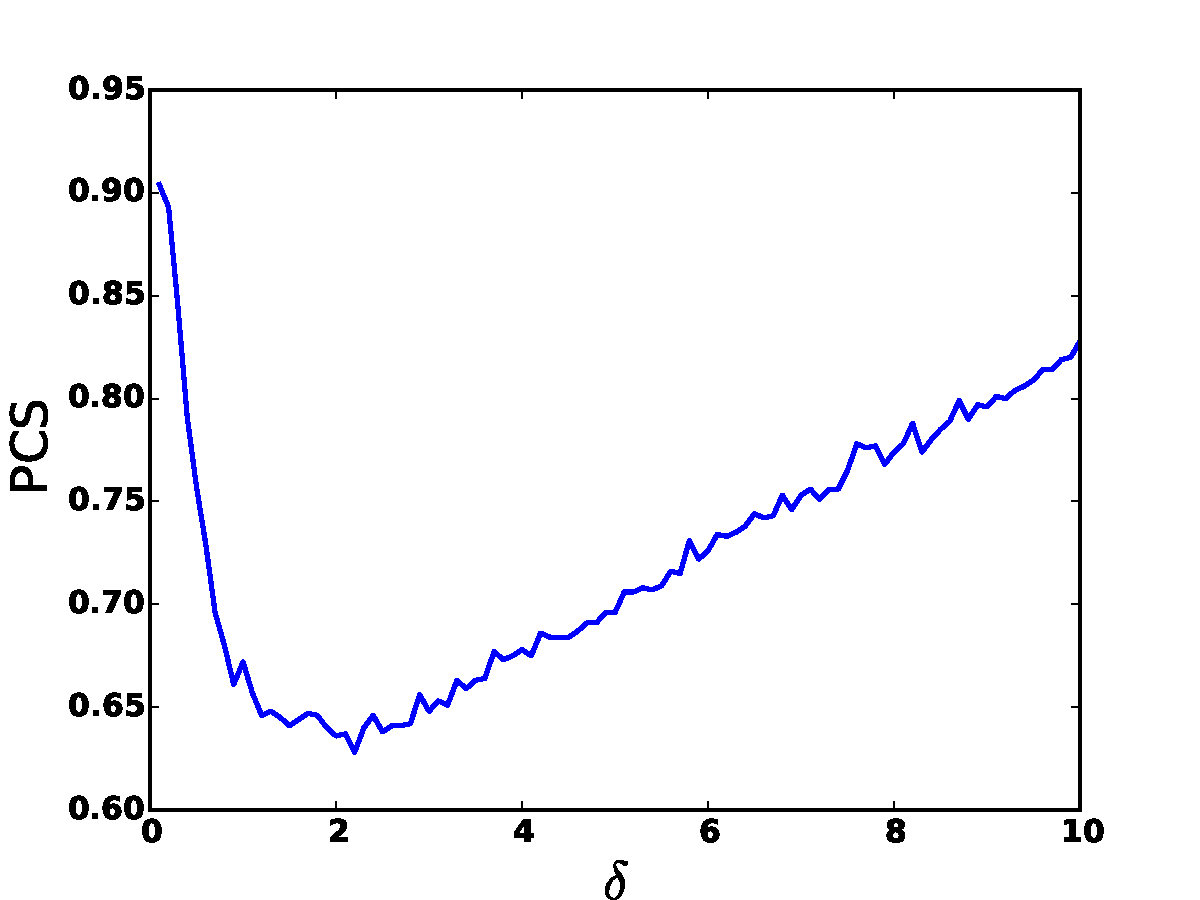
\includegraphics[width=\textwidth,height=0.7\textheight,keepaspectratio]{plot3.pdf}
\caption{
    Known variance case. 100 alternatives and $P^*=0.9$. PCS converges to $P^*$ as $\delta$ goes to $0$. 
    Atypical behavior, $n_0$ is small and the variance of the best alternative is much larger than the other variances.}
\end{figure}
\end{frame}


\begin{frame}{Conclusion}

\begin{block}{}

\begin{itemize}
\item BIZ is a fully sequential IZ procedure with elimination that eliminates
one common source of conservatism: Bonferroni's inequality.\\
\textrm{}\\
\item We have proved the asymptotic validity of the Bayes-inspired Zone
procedure when the variances are known. This implies that BIZ procedure
satisfies the IZ guarantee when the means of the systems are very
similar. \\
\textrm{}\\
\item Theoretical results require unrealistic assumptions on the sampling
variances, but empirical results suggest that behavior is robust to
violations of these assumptions in the problem regimes tested.\\
\textrm{}\\
\end{itemize}
\end{block}

\end{frame}

\begin{frame}{Future Work}

\begin{block}{}

\begin{itemize}
\item Asymptotic validity when the variances are unknown.\\
\textrm{}\\
\item Probability of good selection guarantee: 
\begin{eqnarray*}
\forall\mu,\mbox{ PGS}\left(\mu\right):=\mathbb{P}\left(\mu_{k}-\mu_{\hat{x}}\leq\delta\right) & \geq & P^{*}
\end{eqnarray*}
 \\
\textrm{}\\
\end{itemize}
\end{block}
\end{frame}


\begin{frame}{}


{\Huge{}Thank you!!}\end{frame}

\end{document}
